\documentclass[main.tex]{subfiles}
\begin{document}

\section{Hệ thống các thanh ghi trong 8086}

\begin{figure}[H]
    \centering
    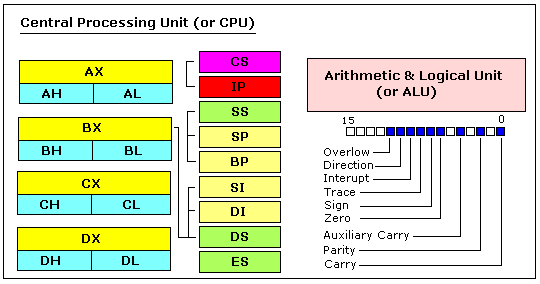
\includegraphics[width=0.8\textwidth]{image/cpu.png}
    \caption{Tổ chức các thanh ghi cơ bản bên trong VXL 8086}
\end{figure}

\subsection{Các thanh ghi đa năng (general purpose registers)}
Vi xử lý 8086 có 8 thanh ghi đa năng gồm:
\begin{itemize}
    \item \cd{AX, BX, CX, DX}: các thanh ghi thường sử dụng nhất. Dùng để chứa các tham số đầu vào cũng như kết quả trả về sau khi thực hiện các lệnh.
    \par 4 thanh ghi này có độ dài 16-bit, mỗi thanh ghi được chia làm 2 thanh ghi nhỏ hơn có độ dài 8-bit là \cd{AH, AL; BH, BL; CH, CL} và \cd{DH, DL}.
    \item \cd{SI} (source index): thanh ghi con trỏ nguồn.
    \item \cd{DI} (destination index): thanh ghi con trỏ đích.
    \item \cd{SP} (stack pointer): thanh ghi trỏ đến đỉnh stack.
    \item \cd{BP} (base pointer): ?
\end{itemize}

Tên của các thanh ghi trên được đặt ra bởi những người tạo ra kiến trúc 8086, tuy nhiên những người lập trình có thể sử dụng chúng tuỳ thích phù hợp với mục đích của mình, nhưng phải tuân theo một số quy luật nhất định.\bigskip

Mỗi thanh ghi trong 4 thanh ghi đa năng \cd{AX, BX, CX, DX} được chia làm 2 phần gọi là high và low. Ví dụ \cd{AX} được cấu thành bởi 2 thành phần là \cd{AH} và \cd{AL}.\\
Giả sử ta có một số thập phân là \cd{12345}. Số này được biểu diễn trong hệ nhị phân là \textcolor{red}{\cd{00110000}}\textcolor{blue}{\cd{00111001}}\cd{b}. Khi ta lưu trữ nó trong thanh ghi \cd{AX}, nó sẽ được chia làm 2 phần như sau:

\begin{figure}[H]
    \centering
    \begin{tikzpicture}[mybox/.style={minimum width=3cm,draw,thick,align=center,minimum height=0.5cm}]
        \node[mybox,label=below:\cd{AH},text=red] (AH) {\cd{00110000}};
        \node[left=1cm of AH] {\cd{AX}};
        \node[right=0pt of AH,mybox,label=below:\cd{AL},text=blue] (AL) {\cd{00111001}};
    
    \end{tikzpicture}
    \caption{Minh hoạ lưu trữ giá trị trong thanh ghi AX.}
\end{figure}

Vì vậy, khi ta thay đổi giá trị của các thanh ghi low và high thì giá trị của thanh ghi lớn cũng bị thay đổi theo và ngược lại.

\subsection{Các thanh ghi đoạn (segment registers)}
\begin{itemize}
    \item \cd{CS} (code segment): trỏ đến đoạn bộ nhớ chứa code thực thi của chương trình.
    \item \cd{DS} (data segment): trỏ đến đoạn bộ nhớ chứa giá trị của các biến cục bộ.
    \item \cd{ES} (extra segment): trỏ đến một đoạn bộ nhớ tuỳ chỉnh. Người sử dụng tự định nghĩa.
    \item \cd{SS} (stack segment): trỏ đến đoạn bộ nhớ chứa call stack của chương trình đang thực thi.
\end{itemize}

Để thuận tiện cho việc quản lý, bộ nhớ vật lý trên máy tính được phân chia thành nhiều khu vực logic khác nhau, được gọi là các \textit{đoạn} (segment), mỗi đoạn có mỗi nhiệm vụ khác nhau. Các vùng nhớ cụ thể bên trong các đoạn được gọi là các \textit{offset}.

Ta có thể hiểu đại khái một ``đoạn'' giống như một con đường, còn một offset nằm trong đoạn đó giống như một số nhà nằm trên con đường đó.

Thanh ghi đoạn được sử dụng phối hợp cùng với các thanh ghi đa năng để ghi lại địa chỉ của các ô nhớ. Khi đó thanh ghi đoạn sẽ được sử dụng để chứa địa chỉ đoạn, còn thanh ghi đa năng sẽ được dùng để chứa địa chỉ lệch (offset) của ô nhớ đó tính từ đầu đoạn. Cả 2 kết hợp lại tạo nên \textit{địa chỉ vật lý} của ô nhớ đó.

\begin{figure}[H]
    \centering
    \begin{tikzpicture}
        \node[] (segment) {\bfseries Đường Nguyễn Trung Trực};
        \node[right=1cm of segment] (offset) {\bfseries Số 56};

        \node[below=1cm of segment,align=center] (segment_desc) {Địa chỉ đoạn};
        \node[below=1cm of offset,align=center] (offset_desc) {Địa chỉ lệch\\ \textit{cái nhà thứ 56 tính từ đầu đường}};

        \draw[->, line width=1pt] (segment_desc) edge (segment);
        \draw[->, line width=1pt] (offset_desc) edge (offset);
    \end{tikzpicture}
\end{figure}

Địa chỉ vật lý (physical address) được tạo thành từ địa chỉ trong chỉ 1 thanh ghi đoạn (segment address) và 1 thanh ghi đa năng (offset address) được tính bằng công thức sau:

\begin{center}
\begin{verbatim}
    physical = segment address * 10h + offset.
\end{verbatim}
\end{center}

Vd: Nếu ta có \cd{segment address = 1230h} và \cd{offset = 45h} (ô nhớ thứ \cd{45h} tính từ đầu đoạn \cd{1230h}) thì địa chỉ vật lý được tạo từ 2 địa chỉ này là \cd{12345h}. Offset còn được gọi là effective address (địa chỉ hiệu quả).\bigskip

Nếu ta có một thanh ghi đoạn là \cd{DS} và một thanh ghi đa năng là \cd{DX} thì địa chỉ vật lý được tạo bởi 2 địa chỉ chứa trong 2 thanh ghi trên được kí hiệu là \cd{DS:DX} và có giá trị là \cd{DS * 10h + DX}. 

Vd: Nếu ta có \cd{DS = 1230h} và \cd{DX = 45h} thì \cd{DS:DX = 12345h}.\bigskip

\textbf{Ý nghĩa của thanh ghi đoạn:} giả sử ta có thanh ghi đoạn \cd{DS} mang giá trị là \cd{1230h} (xem lại định nghĩa của \cd{DS} ở trên). Bên trong chương trình, ta khai báo 3 biến sau, mỗi biến chứa 4 byte dữ liệu.
\begin{minted}[]{c}
    a = 123
    b = 456
    c = 789
\end{minted}
Thì biến \cd a sẽ có offset là \cd 0 (vì nó được khai báo đầu tiên, giống như index \cd 0 của phần tử đầu tiên trong mảng). Do \cd b nằm ngay sau \cd a nên nó sẽ có offset là \cd{0 + 4} (do \cd a có kích thước là 4 byte). Vậy ta cũng có thể suy ra \cd c nằm ở offset số \cd 8.

\begin{figure}[H]
    \centering
    \begin{tikzpicture}[mybox/.style={minimum width=3cm,draw,thick,align=center,minimum height=0.5cm}]
        \node[mybox] (a) {\cd{123d}};
        \node[right=0pt of a, mybox] (b) {\cd{456d}};
        \node[right=0pt of b, mybox] (c) {\cd{789d}};

        \node[anchor=east,left=1cm] (DS) at (a.west) {\cd{DS=1230h}};
        
        \node[anchor=north] (a_label) at (a.south) {\cd{a}};
        \node[anchor=north] (a_offset) at (a_label.south) {\cd{Offset 0}};

        \node[anchor=north] (b_label) at (b.south) {\cd{b}};
        \node[anchor=north] (b_offset) at (b_label.south) {\cd{Offset 4}};

        \node[anchor=north] (c_label) at (c.south) {\cd{c}};
        \node[anchor=north] (c_offset) at (c_label.south) {\cd{Offset 8}};
    
    \end{tikzpicture}
    \caption{Minh hoạ về offset}
\end{figure}

Như vậy địa chỉ vật lý của 3 biến trên lần lượt là:
\begin{table}[H]
    \centering
    \begin{tabular}{|l|l|l|}
    \hline
    Biến        & Offset    & Physical addr.          \\
    \hline
    \cd{a}    & 0         & 1230h * 10h + 0 = 12300h \\
    \cd{b}    & 4         & 1230h * 10h + 4 = 12304h \\
    \cd{c}    & 8         & 1230h * 10h + 8 = 12308h \\
    \hline
    \end{tabular}
\end{table}

\textbf{Vận dụng:} giả sử \cd{a, b, c} mang các kích thước khác nhau lần lượt là \cd{2}, \cd 4 và \cd 6 byte. Hãy cho biết \cd{a, b, c} lần lượt thuộc các offset nào và có địa chỉ vật lý là gì? \\
Đáp án:
\begin{table}[H]
    \centering
    \begin{tabular}{|l|l|l|}
    \hline
    Biến        & Offset    & Physical addr.          \\
    \hline
    \cd{a}    & 0h         & 1230h * 10h + 0h = 12300h \\
    \cd{b}    & 2h         & 1230h * 10h + 2h = 12302h \\
    \cd{c}    & 6h         & 1230h * 10h + 6h = 12306h \\
    \cd{d}    & 12d = Ch   & 1230h * 10h + Ch = 1230Ch \\
    \hline
    \end{tabular}
\end{table}

\subsection{Các thanh ghi đặc biệt (special purpose registers)}
\begin{itemize}
    \item \cd{IP} (instruction pointer): trỏ đến đoạn code đang được thực thi.
    \item Thanh ghi cờ hiệu (flag register): giống như một ``biến toàn cục'' bên trong CPU. Các bit của nó sẽ bị thay đổi giá trị tuỳ thuộc vào kết quả trả về của lệnh mà ta vừa thực hiện trước đó.
\end{itemize}

\subsubsection{Giải thích các bit cờ hiệu phổ biến}
\paragraph{SF (sign flag)}
Sẽ được gán thành \cd 1 nếu most significant bit của kết quả của phép tính vừa thực hiện là \cd 1, hay nói cách khác, kết quả bị âm. Cờ này mang giá trị \cd 0 nếu ngược lại.\break
\textit{Vd:} \cd{01001100b + 01100001b =} \textcolor{red}{\cd 1}\cd{0101101b}.\\ 
Khi đó \cd{SF = 1}.
\bigskip

\paragraph{ZF (zero flag)}
Sẽ được gán thành 1 nếu kết quả của phép tính vừa thực hiện là 0.
\bigskip 

\paragraph{PF (parity flag)}
Sẽ được gán thành \cd 1 nếu trong kết quả của phép tính vừa rồi có một số \textit{chẵn} các bit \cd 1. Nếu không có bit \cd 1 nào thì \cd{PF} cũng bằng \cd 1 (vì 0 cũng là chẵn).\\
\textit{Vd:} \cd{01001100b + 01100001b = 10101101b}. Có 5 bit \cd 1, nên cờ này sẽ mang giá trị \cd 0.

\paragraph{OF (overflow flag)}
\cd{OF} được set thành \cd 1 nếu như 2 số hạng ban đầu có MSB (bit trái nhất) bằng nhau nhưng tổng của 2 số hạng đó có MSB khác kết quả của 2 số hạng ban đầu.
\begin{itemize}
    \item \cdh{1}\cd{111b + }\cdh{1}\cd{000b = } \cdh{0}\cd{000b} $\Rightarrow$ \cd{OF = 1}.
    \item \cdh{0}\cd{111b + }\cdh{0}\cd{001b = }\cdh{1}\cd{111b}. $\Rightarrow$ \cd{OF = 1}.
    \item \cdh{1}\cd{111b + }\cdh{0}\cd{001b = }\cdh{0}\cd{000b}. $\Rightarrow$ \cd{OF = 0}.
\end{itemize}
Overflow flag chỉ bị tác động bởi phép cộng.

\paragraph{CF (carry flag)}
\cd{CF} sẽ mang giá trị \cd 1 trong 2 trường hợp dưới đây:
\begin{itemize}
    \item Khi ta thực hiện phép cộng mà số được nhớ nằm ngoài vùng biểu diễn của thanh ghi.
        \begin{verbatim}
            1111b 
          + 0001b 
            -----
           .0000b 
        \end{verbatim}
    Ta thấy khi ta thực hiện xong phép cộng này, vẫn còn 1 số \cd 1 được ``nhớ'' ở ngoài cùng bên trái, nhưng nó lại nằm ngoài vùng biểu diễn của thanh ghi này (vì nó chỉ có 4 bit).
    \item Khi ta thực hiện phép trừ mà số được ``mượn'' nằm ngoài vùng biểu diễn của thanh ghi.
        \begin{verbatim}
            0000b 
          - 0001b 
            -----
           .1111b 
        \end{verbatim}
    Ta thấy khi ta thực hiện xong phép trừ này, vẫn còn 1 số \cd 1 được ``mượn'' mà chưa trả nằm ở ngoài cùng bên trái của kết quả, nhưng nó lại nằm ngoài vùng biểu diễn của 2 thanh ghi toán hạng, nên ta không thể ``trả'' được.
\end{itemize}

\textit{Lưu ý: CPU không quan tâm phép tính bạn vừa thực hiện là có dấu hay không dấu, 2 số hạng là âm hay dương. Nó chỉ thực hiện việc cộng/trừ trên 2 toán hạng nhị phân và thực hiện việc set cờ tương ứng theo quy luật trên}.\cite{overflow_note}.

\textbf{Một số ví dụ:} 
\begin{figure}[H]
    \centering
    \begin{tabular}{|l|l|l|l|l|l|l|}
    \hline
    Biểu thức                    & SF & ZF & PF & OF & CF \\
    \hline
    \cd{1111b + 1000b = 0000b} & 0  & 1  & 1  & 1  & 1 \\
    \cd{0101b + 0111b = 1100b} & 1  & 0  & 1  & 1  & 0 \\
    \cd{1111b + 0010b = 0001b} & 0  & 0  & 0  & 0  & 1 \\
    \cd{1111b - 0011b = 1100b} & 1  & 0  & 1  & 0  & 0 \\
    \cd{0000b - 0001b = 1111b} & 1  & 0  & 1  & 0  & 1 \\
    \hline
    \end{tabular}
\end{figure}

%%%%%%%%%%%%%%%%%%%%%%%%%%%%%%%%%%%%%%%%%%%%%%%%%%%%%%%

\section{Cấu trúc chung của một chương trình hợp ngữ 8086}
Có rất nhiều cách để tổ chức một chương trình trong 8086 Asm vì sự đa dạng của compiler hồi đó. Tuy nhiên, ta có cách thường sử dụng sau:

\begin{minted}[linenos]{asm}
.model <kiểu bộ nhớ>
.stack <địa chỉ của SS>

.data
    <khai báo các biến>

.code 
    <khai báo các thủ tục và macro>

    main proc 
        <nội dung hàm main>
    endp

end main ; kết thúc chương trình và nhắc compiler tên của hàm main
\end{minted}
Vd: 
\begin{minted}[linenos]{asm}
.model small
.stack 100h

.data
    strHelloWorld db "Hello world$"

.code 
    printDXString proc 
        mov ah, 09h
        int 21h
    endp

    main proc 
        lea dx, strHelloWorld
        call printDXString
    endp

end main 
\end{minted}
\end{document}